% ----------------------------------------------------------------------------
% Setup and configuration
% ----------------------------------------------------------------------------

\documentclass{article}
\usepackage[utf8]{inputenc}

% for serious mathematical typesetting, https://www.ctan.org/pkg/amsmath
\usepackage{amsmath}

% enhances the quality of tables, https://www.ctan.org/pkg/booktabs/
\usepackage{booktabs}

% improve captions that appear above tables
\usepackage{caption}

% use H to place figures and tables at exact location, https://www.ctan.org/pkg/float
\usepackage{float}

% improved graphics capabilities for figures, https://ctan.org/pkg/graphicx
\usepackage{graphicx}

% create hyperlinks in the document and disable border, https://ctan.org/pkg/hyperref
\usepackage[hidelinks]{hyperref}

% write tables that continue to the next page, https://ctan.org/pkg/longtable
\usepackage{longtable}

% greek letters in text without math mode, https://www.ctan.org/pkg/textgreek
\usepackage{textgreek}

% color for text and tables, https://www.ctan.org/pkg/xcolor
\usepackage[table]{xcolor}

% bibliography package and references file, https://www.ctan.org/pkg/biblatex
\usepackage{biblatex}
\addbibresource{references.bib}

% ----------------------------------------------------------------------------
% Document
% ----------------------------------------------------------------------------

\title{Entrained flow reactor (EFR)}
\author{Gavin Wiggins}
\date{\today}

\begin{document}

\maketitle
\tableofcontents

% !TEX root = ../main.tex

\section{Introduction}

This report provides an overview of the Entrained Flow Reactor (EFR) at NREL and associated computational modeling tasks. The reactor operates at fast pyrolysis conditions to thermochemically convert biomass into gaseous products. The EFR is part of the Thermochemical Process Development Unit (TCPDU) at NREL which was originally designed for biomass gasification where the EFR was used as a thermal cracker. An overview of the TCPDU system is shown in Figure \ref{fig:tcpdu-system}.

\begin{figure}[H]
    \centering
    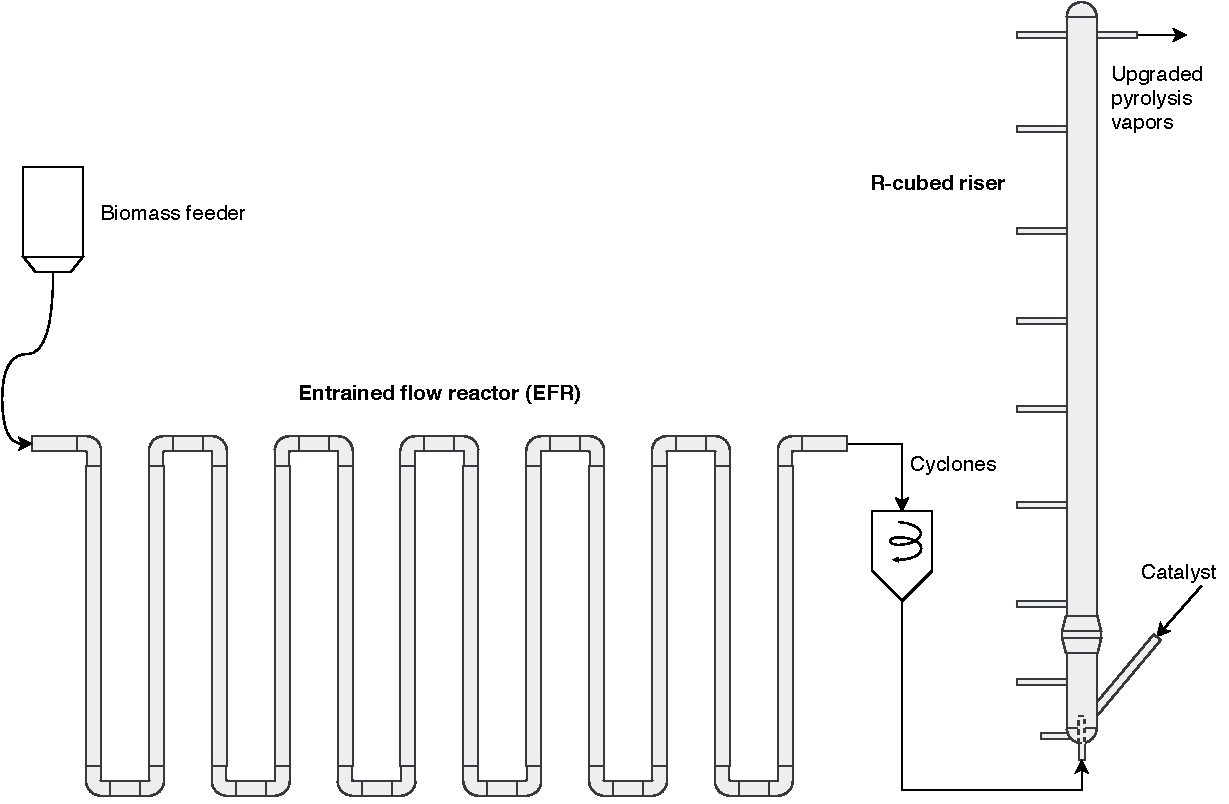
\includegraphics[width=\textwidth]{figures/tcpdu-system.pdf}
    \caption{Overview of the main components of the NREL TCPDU system. Fast pyrolysis of biomass occurs in the entrained flow reactor. Catalytic vapor phase upgrading occurs in the R-cubed riser reactor.}
    \label{fig:tcpdu-system}
\end{figure}

% !TEX root = ../main.tex

\section{Experimental setup}

This section provides geometric dimensions and typical operating conditions for the entrained flow reactor. Characteristics for the Blend3 and forest residue feedstocks are also discussed.

\subsection{Entrained flow reactor}

Fast pyrolysis in the TCPDU system occurs in the entrained flow reactor (EFR) which is comprised of a series of horizontal and vertical pipes connected with 90 degree elbows (see Figure \ref{fig:efr-assembly}). The EFR is essentially a pneumatic conveyor where biomass particles flow through a long pipe with several bends. Dimensions and material information about the EFR are provided in Figure \ref{fig:efr-geometry} below. Operating conditions such as temperatures, pressures, and flow rates for the EFR are shown in Figure \ref{fig:efr-flow}. Nitrogen gas at 500$^{\circ}$C is generally used as the conveying medium for the solids.

\begin{figure}[H]
	\centering
	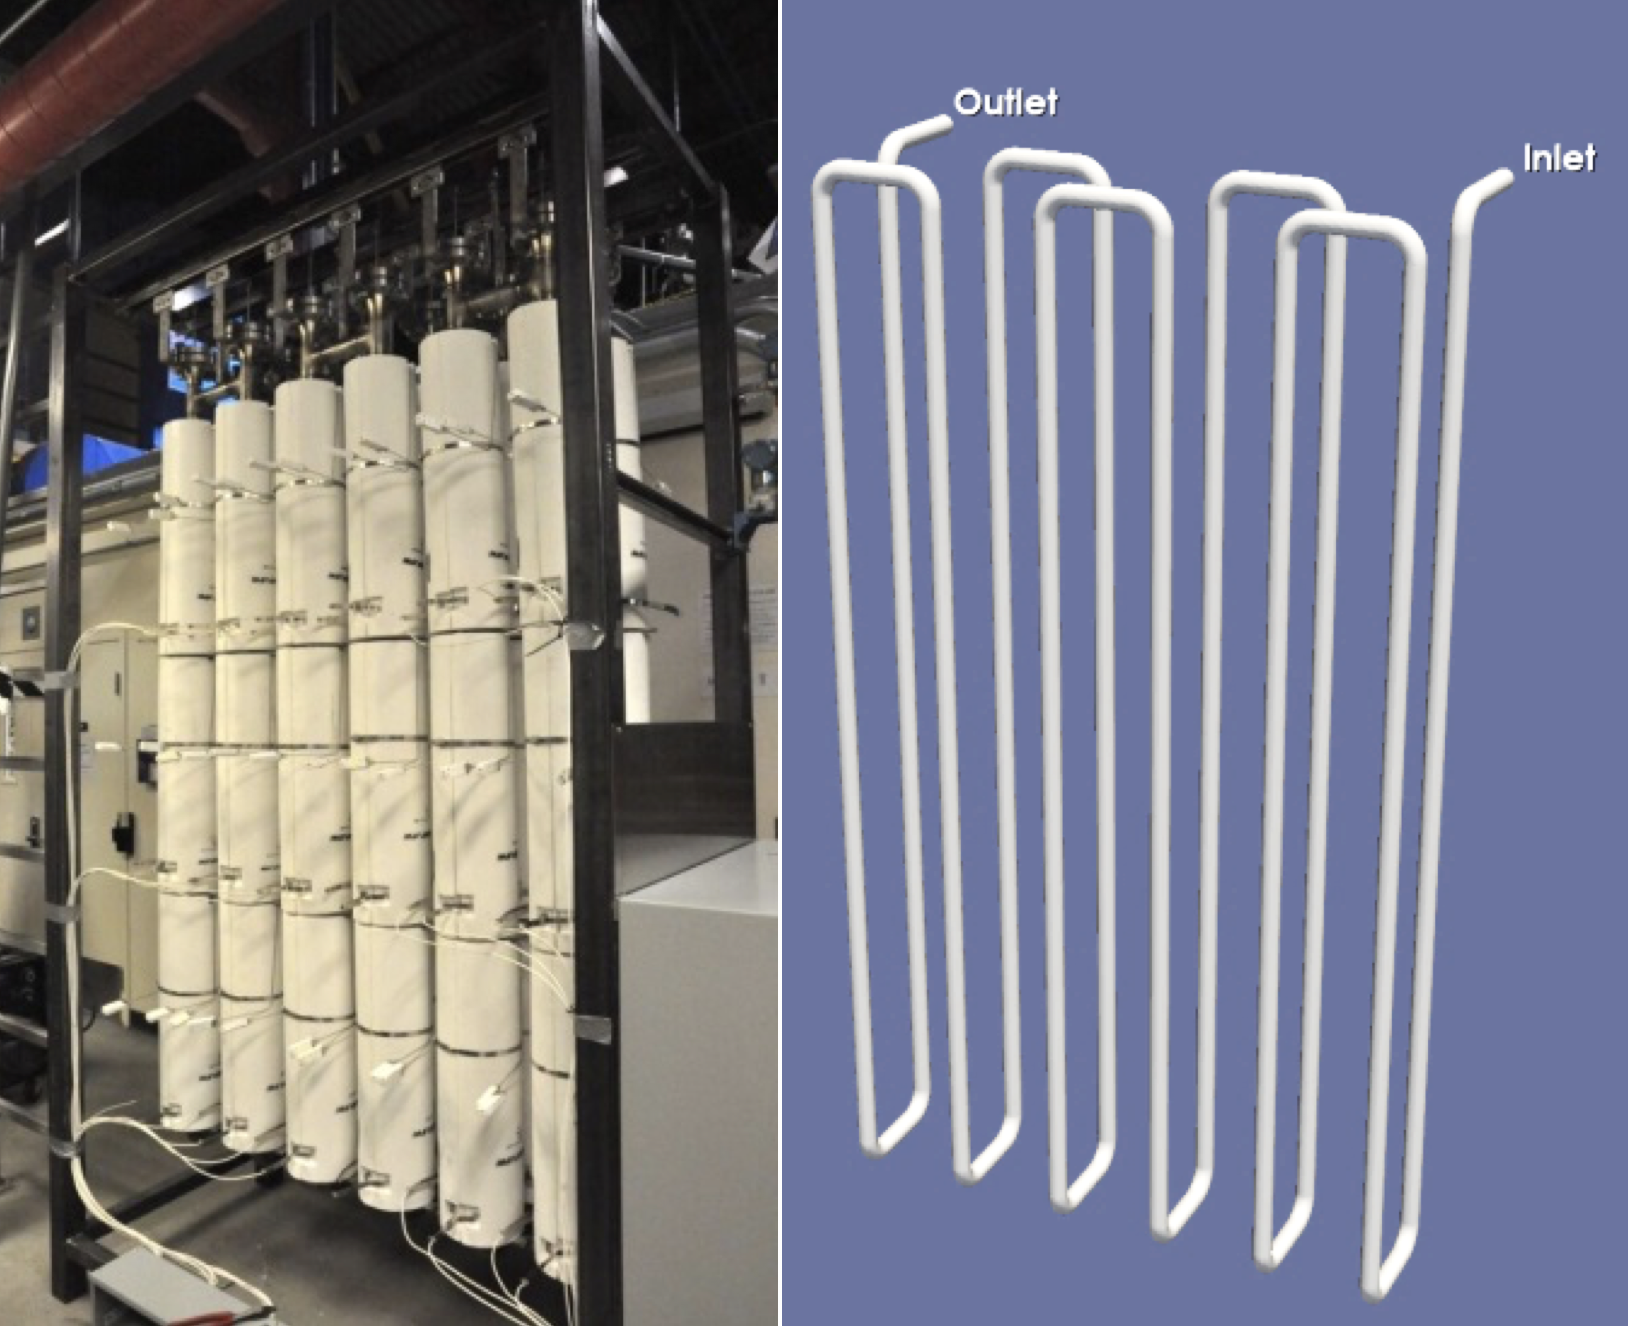
\includegraphics[width=0.8\textwidth]{figures/efr-assembly.png}
	\caption{Left - picture of the EFR assembly with heat jackets, insulation, and thermocouples. Right - CAD representation of the EFR pipe assembly used for MFiX simulations.}
	\label{fig:efr-assembly}
\end{figure}

\begin{figure}[H]
	\centering
	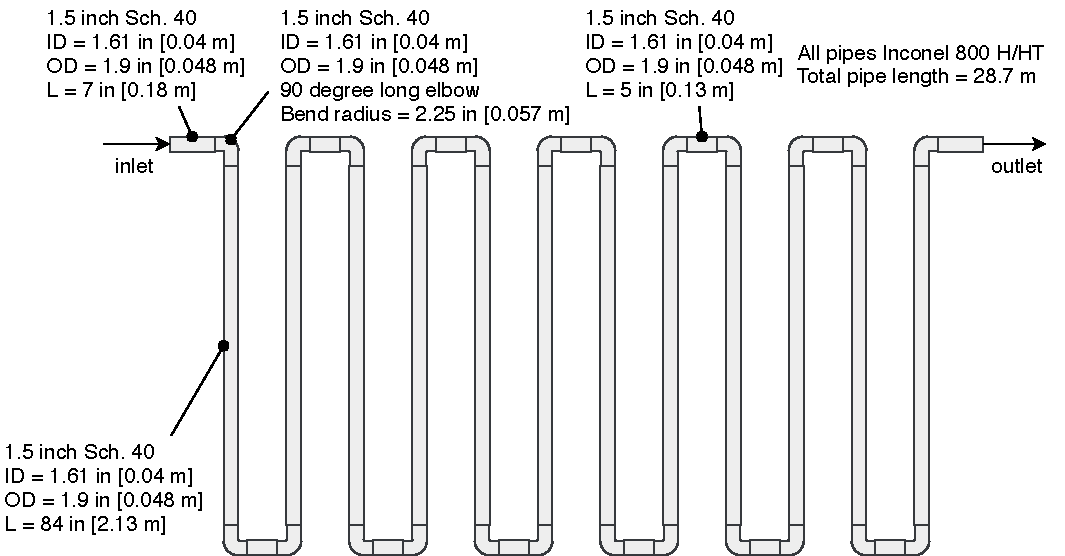
\includegraphics[width=\textwidth]{figures/efr-geometry.pdf}
	\caption{Geometry of the entrained flow reactor at NREL.}
	\label{fig:efr-geometry}
\end{figure}

\begin{figure}[H]
	\centering
	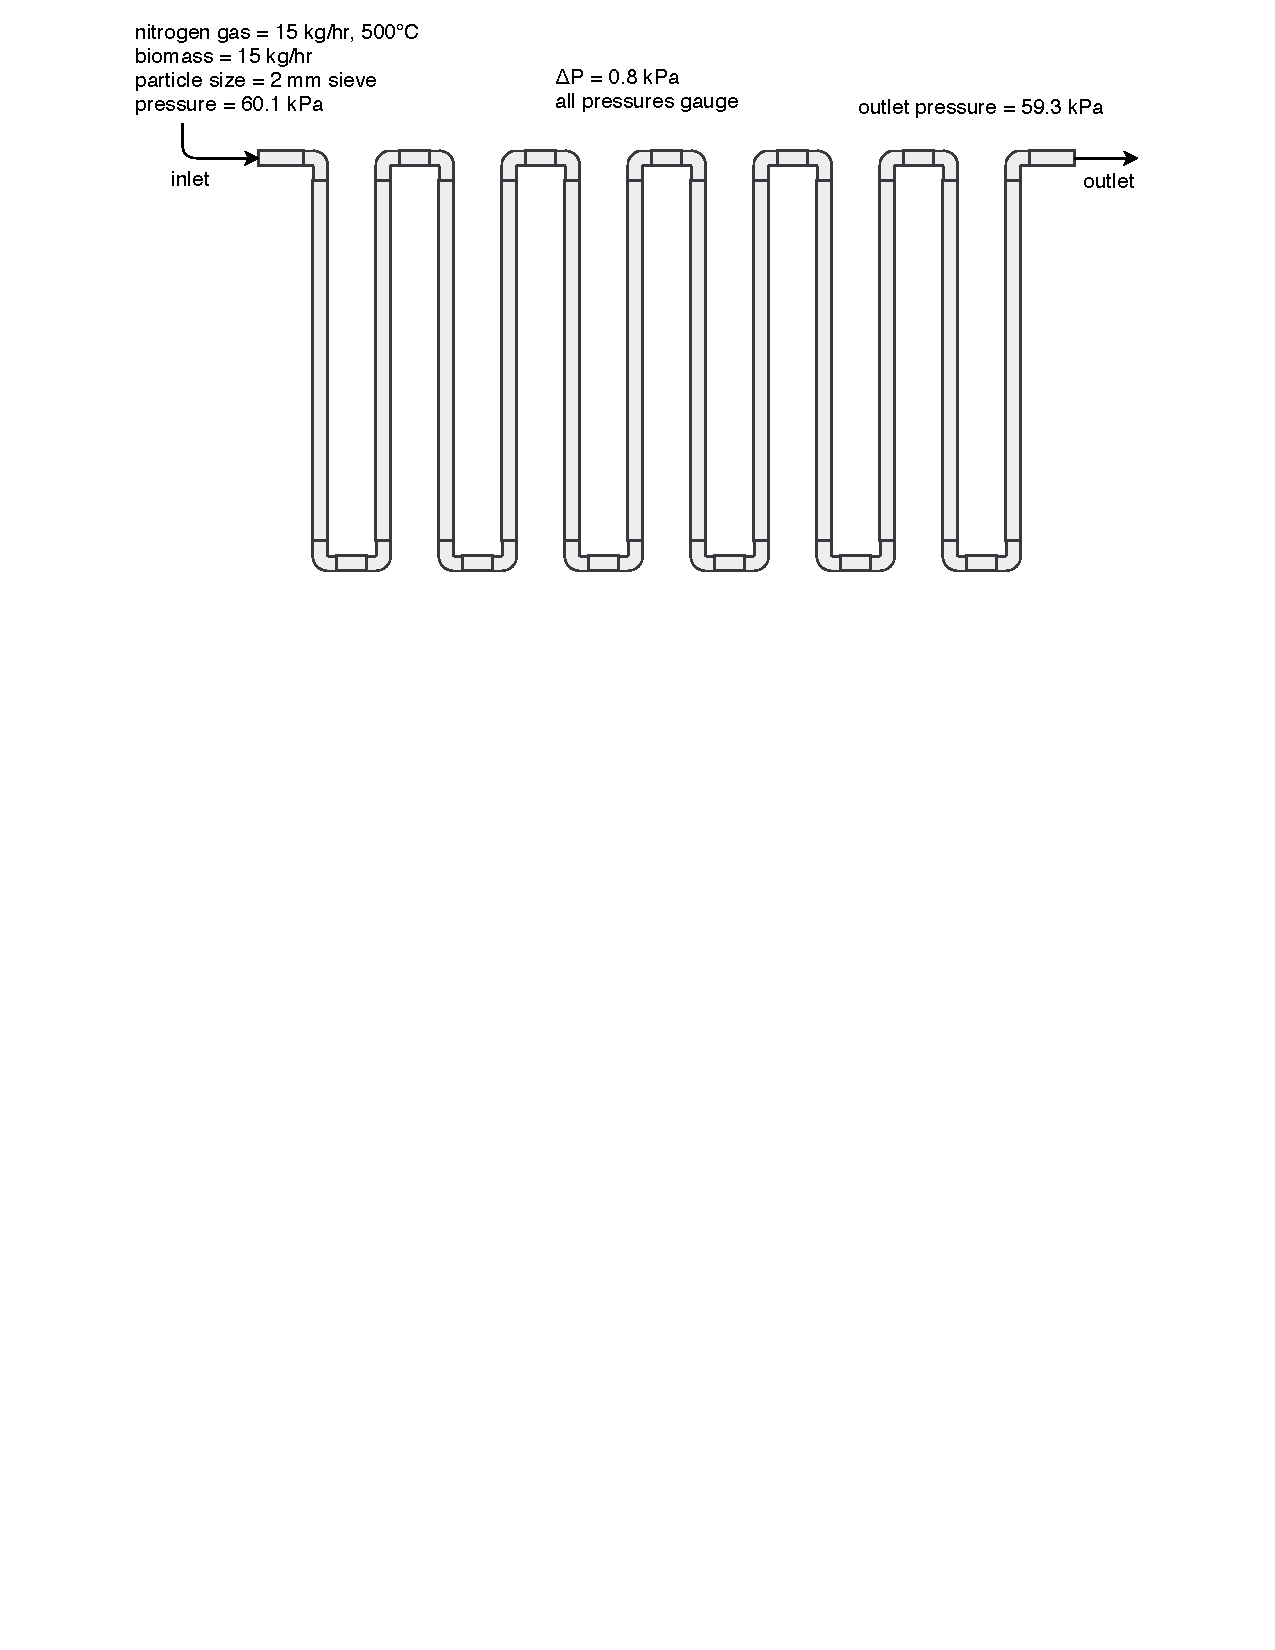
\includegraphics[width=\textwidth]{figures/efr-flow.pdf}
	\caption{Typical operating conditions for the entrained flow reactor.}
	\label{fig:efr-flow}
\end{figure}

\subsection{Blend3 feedstock}

General information about the Blend3 feedstock used in the entrained flow reactor is provided in Table \ref{tab:blend3-info}. There is currently no information regarding identification of the feedstock or who performed the feedstock measurements and data preparation. Proximate and ultimate analysis data for the feedstock are presented in Tables \ref{tab:blend3-prox} and \ref{tab:blend3-ult}. Only one set of analysis data is available therefore the uncertainty in the values is unknown.

\begin{table}[H]
    \centering
    \caption{General information for the Blend3 feedstock.}
    \label{tab:blend3-info}
    \begin{tabular}{ll}
        \toprule
        Item    & Description \\
        \midrule
        Name    & Blend3 \\
        ID      & ? \\
        Contact & ? \\
        \bottomrule
    \end{tabular}
\end{table}

\begin{table}[H]
    \centering
    \caption{Blend3 proximate analysis mass percent, as-received basis. Source \cite{Choratch-2017}.}
    \label{tab:blend3-prox}
    \begin{tabular}{lrrr}
        \toprule
        Proximate & \% ar & \% ar & \% ar \\
        \midrule
        FC        & 16.92 & ? & ? \\
        VM        & 76.40 & ? & ? \\
        ash       & 0.64  & ? & ? \\
        moisture  & 6.04  & ? & ? \\
        \bottomrule
    \end{tabular}
\end{table}

\begin{table}[H]
    \centering
    \caption{Blend3 ultimate analysis mass percent, as-received basis. Source \cite{Choratch-2017}.}
    \label{tab:blend3-ult}
    \begin{tabular}{lrrr}
        \toprule
        Element & \% ar & \% ar & \% ar \\
        \midrule
        C        & 49.52   & ? & ? \\
        H        & 5.28    & ? & ? \\
        O        & 38.35   & ? & ? \\
        N        & 0.15    & ? & ? \\
        S        & 0.02    & ? & ? \\
        ash      & 0.64    & ? & ? \\
        moisture & 6.04    & ? & ? \\
        \bottomrule
    \end{tabular}
\end{table}

The chemical analysis of the Blend3 feedstock is presented in Table \ref{tab:blend3-chem-analysis}. Again, only one set of data is available so the uncertainty in the measurements is unknown. The chemical analysis measurements are used to determine the biomass composition which is needed for the kinetics model.

\begin{table}[H]
    \centering
    \caption{Blend3 chemical analysis mass percent, dry basis. Source \cite{Starace-2020}.}
    \label{tab:blend3-chem-analysis}
    \begin{tabular}{lrrr}
        \toprule
        Chemical component & \% dry & \% dry & \% dry \\
        \midrule
        glucan                    & 38.95 & ? & ? \\
        acetyl                    & 1.59  & ? & ? \\
        arabinan                  & 1.40  & ? & ? \\
        galactan                  & 3.16  & ? & ? \\
        mannan                    & 10.52 & ? & ? \\
        xylan                     & 7.89  & ? & ? \\
        lignin                    & 29.48 & ? & ? \\
        free fructose             & 0.07  & ? & ? \\
        free glucose              & 0.04  & ? & ? \\
        sucrose                   & 0.04  & ? & ? \\
        water extractives         & 2.75  & ? & ? \\
        ethanol extractives       & 3.49  & ? & ? \\
        non-structural inorganics & 0.22  & ? & ? \\
        structural inorganics     & 0.41  & ? & ? \\
        \bottomrule
    \end{tabular}
\end{table}

\begin{table}[H]
    \centering
    \caption{Blend3 ash analysis as weight percent of ash. Source \cite{Choratch-2017}.}
    \begin{tabular}{lrrr}
        \toprule
        Metal oxide & wt. \% & wt. \% & wt. \% \\
        \midrule
        SiO$_2$     & 28.1 & ? & ? \\
        Al$_2$O$_3$ & 7.06 & ? & ? \\
        TiO$_2$     & 0.34 & ? & ? \\
        CaO         & 21.8 & ? & ? \\
        Na$_2$O     & 0.71 & ? & ? \\
        K$_2$O      & 13.8 & ? & ? \\
        P$_2$O$_5$  & 5.47 & ? & ? \\
        SO$_3$      & 1.23 & ? & ? \\
        Cl          & 0.09 & ? & ? \\
        CO$_2$      & 5.14 & ? & ? \\
        \bottomrule
    \end{tabular}
\end{table}

\begin{table}[H]
    \centering
    \caption{Blend3 particle properties from pelletized crushed feedstock. The crushed feedstock is used in the entrained flow reactor.}
    \begin{tabular}{crlc}
        \toprule
        Property & Value & Description & Source \\
        \midrule
        $\rho$  & 1,050 kg/m$^3$ & particle density, daf basis & \cite{Pecha-2018} \\
        $\eta$  & 0.27           & particle porosity & \\
        $k$     & 0.23 W/mK      & thermal conductivity & \\
        \bottomrule
    \end{tabular}
\end{table}

\begin{table}[H]
    \centering
    \caption{Entrained flow reactor yields for Blend3 feedstock.}
    \begin{tabular}{lr}
        \toprule
        Yield & wt. \% \\
        \midrule
        total liquid   & 64.9 \\
        char           & 13.9 $\pm$ 0.1 \\
        gas            & 17.2 $\pm$ 0.2 \\
        mass balance   & 96.9 $\pm$ 1.5 \\
        carbon balance & 93.0 $\pm$ 1.0 \\
        \bottomrule
    \end{tabular}
\end{table}

\subsection{Forest residue feedstock}

The forest residue feedstock is comprised of branches/twigs, cambium, needles, bark, and whitewood. This feedstock is used in the NREL fluidized bed reactor (FBR) for the purposes of the FCIC project. The FBR is operated at fast pyrolysis conditions for the thermochemical conversion of biomass. The reactor is sometimes referred to as the 2FBR.

\begin{table}[H]
    \centering
    \caption{General information for the forest residue feedstock.}
    \begin{tabular}{ll}
        \toprule
        Item    & Description \\
        \midrule
        Name    & forest residue \\
        ID      & ? \\
        Contact & ? \\
        \bottomrule
    \end{tabular}
\end{table}

\begin{table}[H]
    \centering
    \caption{Bark ultimate analysis mass percent, dry ash-free basis. Source \cite{Unknown-2019}.}
    \begin{tabular}{lrrr}
        \toprule
        Element & \% daf & \% daf & \% daf \\
        \midrule
        C        & 48.27 & ? & ? \\
        H        & 5.72  & ? & ? \\
        N        & 0.52  & ? & ? \\
        \bottomrule
    \end{tabular}
\end{table}

\begin{table}[H]
    \centering
    \caption{Branches/twigs ultimate analysis mass percent, dry ash-free basis. Source \cite{Unknown-2019}.}
    \begin{tabular}{lrrr}
        \toprule
        Element & \% daf & \% daf & \% daf \\
        \midrule
        C        & 49.69 & ? & ? \\
        H        & 6.36  & ? & ? \\
        N        & 0.25  & ? & ? \\
        \bottomrule
    \end{tabular}
\end{table}

\begin{table}[H]
    \centering
    \caption{Cambium ultimate analysis mass percent, dry ash-free basis. Source \cite{Unknown-2019}.}
    \begin{tabular}{lrrr}
        \toprule
        Element & \% daf & \% daf & \% daf \\
        \midrule
        C        & 48.52 & ? & ? \\
        H        & 6.39  & ? & ? \\
        N        & 0.11  & ? & ? \\
        \bottomrule
    \end{tabular}
\end{table}

\begin{table}[H]
    \centering
    \caption{Needles ultimate analysis mass percent, dry ash-free basis. Source \cite{Unknown-2019}.}
    \begin{tabular}{lrrr}
        \toprule
        Element & \% daf & \% daf & \% daf \\
        \midrule
        C        & 48.59 & ? & ? \\
        H        & 5.92  & ? & ? \\
        N        & 1.22  & ? & ? \\
        \bottomrule
    \end{tabular}
\end{table}

\begin{table}[H]
    \centering
    \caption{Whitewood ultimate analysis mass percent, dry ash-free basis. Source \cite{Unknown-2019}.}
    \begin{tabular}{lrrr}
        \toprule
        Element & \% daf & \% daf & \% daf \\
        \midrule
        C        & 48.27 & ? & ? \\
        H        & 6.15  & ? & ? \\
        N        & 0.10  & ? & ? \\
        \bottomrule
    \end{tabular}
\end{table}

\begin{table}[H]
    \centering
    \caption{Whitewood biomass composition mass percent, dry basis. Source \cite{Unknown-2020}.}
    \begin{tabular}{lr}
        \toprule
        Component & \% dry \\
        \midrule
        Cellulose       & 38.04 \\
        Hemicellulose   & 24.2  \\
        \bottomrule
    \end{tabular}
\end{table}

% !TEX root = ../main.tex

\section{Model development}

Details about the biomass pyrolysis kinetics and computational models developed for the entrained flow reactor are discussed in this section.

\subsection{Pyrolysis kinetics}

The kinetic reaction mechanisms presented by Debiagi et al. are used to model biomass pyrolysis in the entrained flow reactor. These reactions are shown below in Table \ref{tab:chem-kinetics}.

\begin{center}
    \footnotesize
    \setlength\LTleft{-1in}
    \setlength\LTright{-1in}
    \begin{longtable}{cp{4in}lr}
        \caption{Kinetic reactions for biomass pyrolysis where A is the prefactor, E is the activation energy, and T is temperature. Source \cite{Debiagi-2018}.}
        \label{tab:chem-kinetics} \\
        \toprule
        Item & Reaction & A (1/s) & E (cal/mol) \\
        \midrule
        1  & CELL $\rightarrow$ CELLA & 1.5 $\times$ 10$^{14}$ & 47,000 \\
        2  & CELLA $\rightarrow$ 0.40 CH2OHCHO + 0.03 CHOCHO + 0.17 CH3CHO + 0.25 C6H6O3 + 0.35 C2H5CHO + 0.20 CH3OH + 0.15 CH2O + 0.49 CO + 0.05 G\{CO\} + 0.43 CO2 + 0.13 H2 + 0.93 H2O + 0.05 G\{COH2\} loose + 0.02 HCOOH + 0.05 CH2OHCH2CHO + 0.05 CH4 + 0.1 G\{H2\} + 0.66 CHAR & 2.5 $\times$ 10$^6$ & 19,100 \\
        3  & CELLA $\rightarrow$ C6H10O5 & 3.3 $\times$ T & 10,000 \\
        4  & CELL $\rightarrow$ 4.45 H2O + 5.45 CHAR + 0.12 G\{COH2\} stiff + 0.18 G\{COH2\} loose + 0.25 G\{CO\} + 0.125 G\{H2\} + 0.125 H2 & 9.0 $\times$ 10$^7$ & 31,000 \\
        5  & GMSW $\rightarrow$ 0.70 HCE1 + 0.30 HCE2 & 1.0 $\times$ 10$^{10}$ & 31,000 \\
        6  & XYHW $\rightarrow$ 0.35 HCE1 + 0.65 HCE2 & 1.25 $\times$ 10$^{11}$ & 31,400 \\
        7  & XYGR $\rightarrow$ 0.12 HCE1 + 0.88 HCE2 & 1.25 $\times$ 10$^{11}$ & 30,000 \\
        8  & HCE1 $\rightarrow$ 0.25 C5H8O4 + 0.25 C6H10O5 + 0.16 FURFURAL + 0.13 C6H6O3 + 0.09 CO2 + 0.1 CH4 + 0.54 H2O + 0.06 CH2OHCH2CHO + 0.1 CHOCHO + 0.02 H2 + 0.1 CHAR & 16.0 $\times$ T & 12,900 \\
        9  & HCE1 $\rightarrow$ 0.4 H2O + 0.39 CO2 + 0.05 HCOOH + 0.49 CO + 0.01 G\{CO\} + 0.51 G\{CO2\} + 0.05 G\{H2\} + 0.4 CH2O + 0.43 G\{COH2\} loose + 0.3 CH4 + 0.325 G\{CH4\} + 0.1 C2H4 + 0.075 G\{C2H4\} + 0.975 CHAR + 0.37 G\{COH2\} stiff + 0.1 H2 + 0.2 G\{C2H6\} & 3.0 $\times$ 10$^{-3}$ $\times$ T & 3,600 \\
        10 & HCE2 $\rightarrow$ 0.3 CO + 0.5125 CO2 + 0.1895 CH4 + 0.5505 H2 + 0.056 H2O + 0.049 C2H5OH + 0.035 CH2OHCHO + 0.105 CH3CO2H + 0.0175 HCOOH + 0.145 FURFURAL + 0.05 G\{CH4\} + 0.105 G\{CH3OH\} + 0.1 G\{C2H4\} + 0.45 G\{CO2\} + 0.18 G\{COH2\} loose + 0.7125 CHAR + 0.21 G\{H2\} + 0.78 G\{COH2\} stiff + 0.2 G\{C2H6\} & 7.0 $\times$ 10$^9$ & 30,500 \\
        11 & LIGH $\rightarrow$ LIGOH + 0.5 C2H5CHO + 0.4 C2H4 + 0.2 CH2OHCHO + 0.1 CO + 0.1 C2H6 & 6.7 $\times$ 10$^{12}$ & 37,500 \\
        12 & LIGO $\rightarrow$ LIGOH + CO2 & 3.3 $\times$ 10$^8$ & 25,500 \\
        13 & LIGC $\rightarrow$ 0.35 LIGCC + 0.1 VANILLIN + 0.1 C6H5OCH3 + 0.27 C2H4 + H2O + 0.17 G\{COH2\} loose + 0.4 G\{COH2\} stiff + 0.22 CH2O + 0.21 CO + 0.1 CO2 + 0.36 G\{CH4\} + 5.85 CHAR + 0.2 G\{C2H6\} + 0.1 G\{H2\} & 1.0 $\times$ 10$^{11}$ & 37,200 \\
        14 & LIGCC $\rightarrow$ 0.25 VANILLIN + 0.15 CRESOL + 0.15 C6H5OCH3 + 0.35 CH2OHCHO + 0.7 H2O + 0.45 CH4 + 0.3 C2H4 + 0.7 H2 + 1.15 CO + 0.4 G\{CO\} + 6.80 CHAR + 0.4 C2H6 & 1.0 $\times$ 10$^4$ & 24,800 \\
        15 & LIGOH $\rightarrow$ 0.9 LIG + H2O + 0.1 CH4 + 0.6 CH3OH + 0.3 G\{CH3OH\} + 0.05 CO2 + 0.65 CO + 0.6 G\{CO\} + 0.05 HCOOH + 0.45 G\{COH2\} loose + 0.4 G\{COH2\} stiff + 0.25 G\{CH4\} + 0.1 G\{C2H4\} + 0.15 G\{C2H6\} + 4.25 CHAR + 0.025 C24H28O4 + 0.1 C2H3CHO & 1.5 $\times$ 10$^8$ & 30,000 \\
        16 & LIG $\rightarrow$ VANILLIN + 0.1 C6H5OCH3 + 0.5 C2H4 + 0.6 CO + 0.3 CH3CHO + 0.1 CHAR & 4.0 $\times$ T & 12,000 \\
        17 & LIG $\rightarrow$ 0.6 H2O + 0.3 CO + 0.1 CO2 + 0.2 CH4 + 0.4 CH2O + 0.2 G\{CO\} + 0.4 G\{CH4\} + 0.5 G\{C2H4\} + 0.4 G\{CH3OH\} + 1.25 G\{COH2\} loose + 0.65 G\{COH2\} stiff + 6.1 CHAR + 0.1 G\{H2\} & 8.3 $\times$ 10$^{-2}$ $\times$ T & 8,000 \\
        18 & LIG $\rightarrow$ 0.6 H2O + 2.6 CO + 0.6 CH4 + 0.4 CH2O + 0.75 C2H4 + 0.4 CH3OH + 4.5 CHAR + 0.5 C2H6 & 1.5 $\times$ 10$^9$ & 31,500 \\
        19 & TGL $\rightarrow$ C2H3CHO + 2.5 MLINO + 0.5 U2ME12 & 7.0 $\times$ 10$^{12}$ & 45,700 \\
        20 & TANN $\rightarrow$ 0.85 C6H5OH + 0.15 G\{C6H5OH\} + G\{CO\} + H2O + ITANN & 2.0 $\times$ 10$^1$ & 10,000 \\
        21 & ITANN $\rightarrow$ 5 CHAR + 2 CO + H2O + 0.55 G\{COH2\} loose + 0.45 G\{COH2\} stiff & 1.0 $\times$ 10$^3$ & 25,000 \\
        22 & G\{CO2\} $\rightarrow$ CO2 & 1.0 $\times$ 10$^6$ & 24,500 \\
        23 & G\{CO\} $\rightarrow$ CO & 5.0 $\times$ 10$^{12}$ & 52,500 \\
        24 & G\{CH3OH\} $\rightarrow$ CH3OH & 2.0 $\times$ 10$^{12}$ & 50,000 \\
        25 & G\{COH2\}loose $\rightarrow$ 0.2 CO + 0.2 H2 + 0.8 H2O + 0.8 CHAR & 6.0 $\times$ 10$^{10}$ & 50,000 \\
        26 & G\{C2H6\} $\rightarrow$ C2H6 & 1.0 $\times$ 10$^{11}$ & 52,000 \\
        27 & G\{CH4\} $\rightarrow$ CH4 & 1.0 $\times$ 10$^{11}$ & 53,000 \\
        28 & G\{C2H4\} $\rightarrow$ C2H4 & 1.0 $\times$ 10$^{11}$ & 54,000 \\
        29 & G\{C6H5OH\} $\rightarrow$ C6H5OH & 1.5 $\times$ 10$^{12}$ & 55,000 \\
        30 & G\{COH2\}stiff $\rightarrow$ 0.8 CO + 0.8 H2 + 0.2 H2O + 0.2 CHAR & 1.0 $\times$ 10$^9$ & 59,000 \\
        31 & G\{H2\} $\rightarrow$ H2 & 1.0 $\times$ 10$^8$ & 70,000 \\
        32 & ACQUA $\rightarrow$ H2O & 1.0 $\times$ T & 8,000 \\
        \bottomrule
    \end{longtable}
\end{center}

Chemical species in the Debiagi et al. kinetic scheme for biomass pyrolysis are listed in Table \ref{tab:chem-species}. Species are grouped into solid, metaplastic, gas, and liquid phases.

\begin{center}
    \footnotesize
    \begin{longtable}{cllll}
        \caption{Chemical species in the Debiagi kinetics scheme for biomass pyrolysis. Source \cite{Debiagi-2018}.}
        \label{tab:chem-species} \\
        \toprule
        Item & Name & Formula & Phase & Description \\
        \midrule
        1  & CELL           & C$_6$H$_{10}$O$_5$      & \cellcolor{green!25}solid        & cellulose \\
        2  & CELLA          & C$_6$H$_{10}$O$_5$      & \cellcolor{green!25}solid        & active cellulose \\
        3  & GMSW           & C$_5$H$_{8}$O$_4$       & \cellcolor{green!25}solid        & hemicellulose softwood \\
        4  & XYHW           & C$_5$H$_{8}$O$_4$       & \cellcolor{green!25}solid        & hemicellulose hardwood \\
        5  & XYGR           & C$_5$H$_{8}$O$_4$       & \cellcolor{green!25}solid        & hemicellulose grass \\
        6  & HCE1           & C$_5$H$_{8}$O$_4$       & \cellcolor{green!25}solid        & intermediate hemicellulose \\
        7  & HCE2           & C$_5$H$_{8}$O$_4$       & \cellcolor{green!25}solid        & intermediate hemicellulose \\
        8  & ITANN          & C$_8$H$_{4}$O$_4$       & \cellcolor{green!25}solid        & intermediate phenolics \\
        9  & LIG            & C$_{11}$H$_{12}$O$_4$   & \cellcolor{green!25}solid        & intermediate lignin \\
        10 & LIGC           & C$_{15}$H$_{14}$O$_4$   & \cellcolor{green!25}solid        & carbon rich lignin \\
        11 & LIGCC          & C$_{15}$H$_{14}$O$_4$   & \cellcolor{green!25}solid        & intermediate lignin \\
        12 & LIGH           & C$_{22}$H$_{28}$O$_9$   & \cellcolor{green!25}solid        & hydrogen rich lignin \\
        13 & LIGO           & C$_{20}$H$_{22}$O$_{10}$& \cellcolor{green!25}solid        & oxygen rich lignin \\
        14 & LIGOH          & C$_{19}$H$_{22}$O$_8$   & \cellcolor{green!25}solid        & intermediate lignin \\
        15 & TANN           & C$_{15}$H$_{12}$O$_7$   & \cellcolor{green!25}solid        & tannins \\
        16 & TGL            & C$_{57}$H$_{100}$O$_7$  & \cellcolor{green!25}solid        & triglycerides \\
        17 & CHAR           & C                       & \cellcolor{green!25}solid        & char as pure carbon \\
        18 & G\{COH2\} loose& CH$_2$O                 & \cellcolor{orange!25}metaplastic & loose formaldehyde \\
        19 & G\{CO2\}       & CO$_2$                  & \cellcolor{orange!25}metaplastic & trapped carbon dioxide \\
        20 & G\{CO\}        & CO                      & \cellcolor{orange!25}metaplastic & trapped carbon monoxide \\
        21 & G\{CH3OH\}     & CH$_4$O                 & \cellcolor{orange!25}metaplastic & trapped methanol \\
        22 & G\{CH4\}       & CH$_4$                  & \cellcolor{orange!25}metaplastic & trapped methane \\
        23 & G\{C2H4\}      & C$_2$H$_4$              & \cellcolor{orange!25}metaplastic & trapped ethylene \\
        24 & G\{C6H5OH\}    & C$_6$H$_6$O             & \cellcolor{orange!25}metaplastic & trapped phenol \\
        25 & G\{COH2\} stiff& CH$_2$O                 & \cellcolor{orange!25}metaplastic & stiff formaldehyde \\
        26 & G\{H2\}        & H$_2$                   & \cellcolor{orange!25}metaplastic & trapped hydrogen \\
        27 & G\{C2H6\}      & C$_2$H$_6$              & \cellcolor{orange!25}metaplastic & trapped ethane \\
        28 & C2H4           & C$_2$H$_4$              & \cellcolor{purple!25}gas         & ethylene \\
        29 & C2H6           & C$_2$H$_6$              & \cellcolor{purple!25}gas         & ethane \\
        30 & CH2O           & CH$_2$O                 & \cellcolor{purple!25}gas         & formaldehyde \\
        31 & CH4            & CH$_4$                  & \cellcolor{purple!25}gas         & methane \\
        32 & CO             & CO                      & \cellcolor{purple!25}gas         & carbon monoxide \\
        33 & CO2            & CO$_2$                  & \cellcolor{purple!25}gas         & carbon dioxide \\
        34 & H2             & H$_2$                   & \cellcolor{purple!25}gas         & hydrogen \\
        35 & C2H3CHO        & C$_3$H$_4$O             & \cellcolor{blue!25}liquid        & acrolein \\
        36 & C2H5CHO        & C$_3$H$_6$O             & \cellcolor{blue!25}liquid        & propionaldehyde \\
        37 & C2H5OH         & C$_2$H$_6$O             & \cellcolor{blue!25}liquid        & ethanol \\
        38 & C5H8O4         & C$_5$H$_8$O$_4$         & \cellcolor{blue!25}liquid        & xylofuranose \\
        39 & C6H10O5        & C$_6$H$_{10}$O$_5$      & \cellcolor{blue!25}liquid        & levoglucosan \\
        40 & C6H5OCH3       & C$_7$H$_8$O             & \cellcolor{blue!25}liquid        & anisole \\
        41 & C6H5OH         & C$_6$H$_6$O             & \cellcolor{blue!25}liquid        & phenol \\
        42 & C6H6O3         & C$_6$H$_6$O$_3$         & \cellcolor{blue!25}liquid        & hydroxymethylfurfural \\
        43 & C24H28O4       & C$_{24}$H$_{28}$O$_4$   & \cellcolor{blue!25}liquid        & heavy molecular weight lignin \\
        44 & CH2OHCH2CHO    & C$_3$H$_6$O$_2$         & \cellcolor{blue!25}liquid        & propionic acid \\
        45 & CH2OHCHO       & C$_2$H$_4$O$_2$         & \cellcolor{blue!25}liquid        & acetic acid \\
        46 & CH3CHO         & C$_2$H$_4$O             & \cellcolor{blue!25}liquid        & acetaldehyde \\
        47 & CH3CO2H        & C$_2$H$_4$O$_2$         & \cellcolor{blue!25}liquid        & acetic acid \\
        48 & CH3OH          & CH$_4$O                 & \cellcolor{blue!25}liquid        & methanol \\
        49 & CHOCHO         & C$_2$H$_2$O$_2$         & \cellcolor{blue!25}liquid        & glyoxal \\
        50 & CRESOL         & C$_7$H$_8$O             & \cellcolor{blue!25}liquid        & cresol \\
        51 & FURFURAL       & C$_5$H$_4$O$_2$         & \cellcolor{blue!25}liquid        & 2-furaldehyde \\
        52 & H2O            & H$_2$O                  & \cellcolor{blue!25}liquid        & water from reactions \\
        53 & HCOOH          & CH$_2$O$_2$             & \cellcolor{blue!25}liquid        & formic acid \\
        54 & MLINO          & C$_{19}$H$_{34}$O$_2$   & \cellcolor{blue!25}liquid        & methyl linoleate \\
        55 & U2ME12         & C$_{13}$H$_{22}$O$_2$   & \cellcolor{blue!25}liquid        & linalyl propionate \\
        56 & VANILLIN       & C$_8$H$_8$O$_3$         & \cellcolor{blue!25}liquid        & vanillin \\
        57 & ACQUA          & H$_2$O                  & \cellcolor{blue!25}liquid        & water within biomass \\
        \bottomrule
    \end{longtable}
\end{center}

\subsection{Biomass characterization}

Here.

\begin{table}[H]
    \centering
    \caption{Blend3 biomass composition mass percent, dry basis. Values are calculated from Table \ref{tab:chem-analysis}.}
    \begin{tabular}{lr}
        \toprule
        Biomass composition & \% dry \\
        \midrule
        cellulose     & 38.95 \\
        hemicellulose & 24.56 \\
        lignin        & 29.48 \\
        tann          & 2.90  \\
        tgl           & 3.49  \\
        ash           & 0.63  \\
        \bottomrule
    \end{tabular}
\end{table}

\subsection{Sensitivity analysis}

Here.

% !TEX root = ../main.tex

\section{Results and discussion}

Here.

\subsection{Sensitivity analysis}

Results for the sensitivity analysis of the Debiagi kinetics using a batch reactor model are shown in Tables X.

\begin{figure}[H]
    \centering
    \makebox[\textwidth][c]{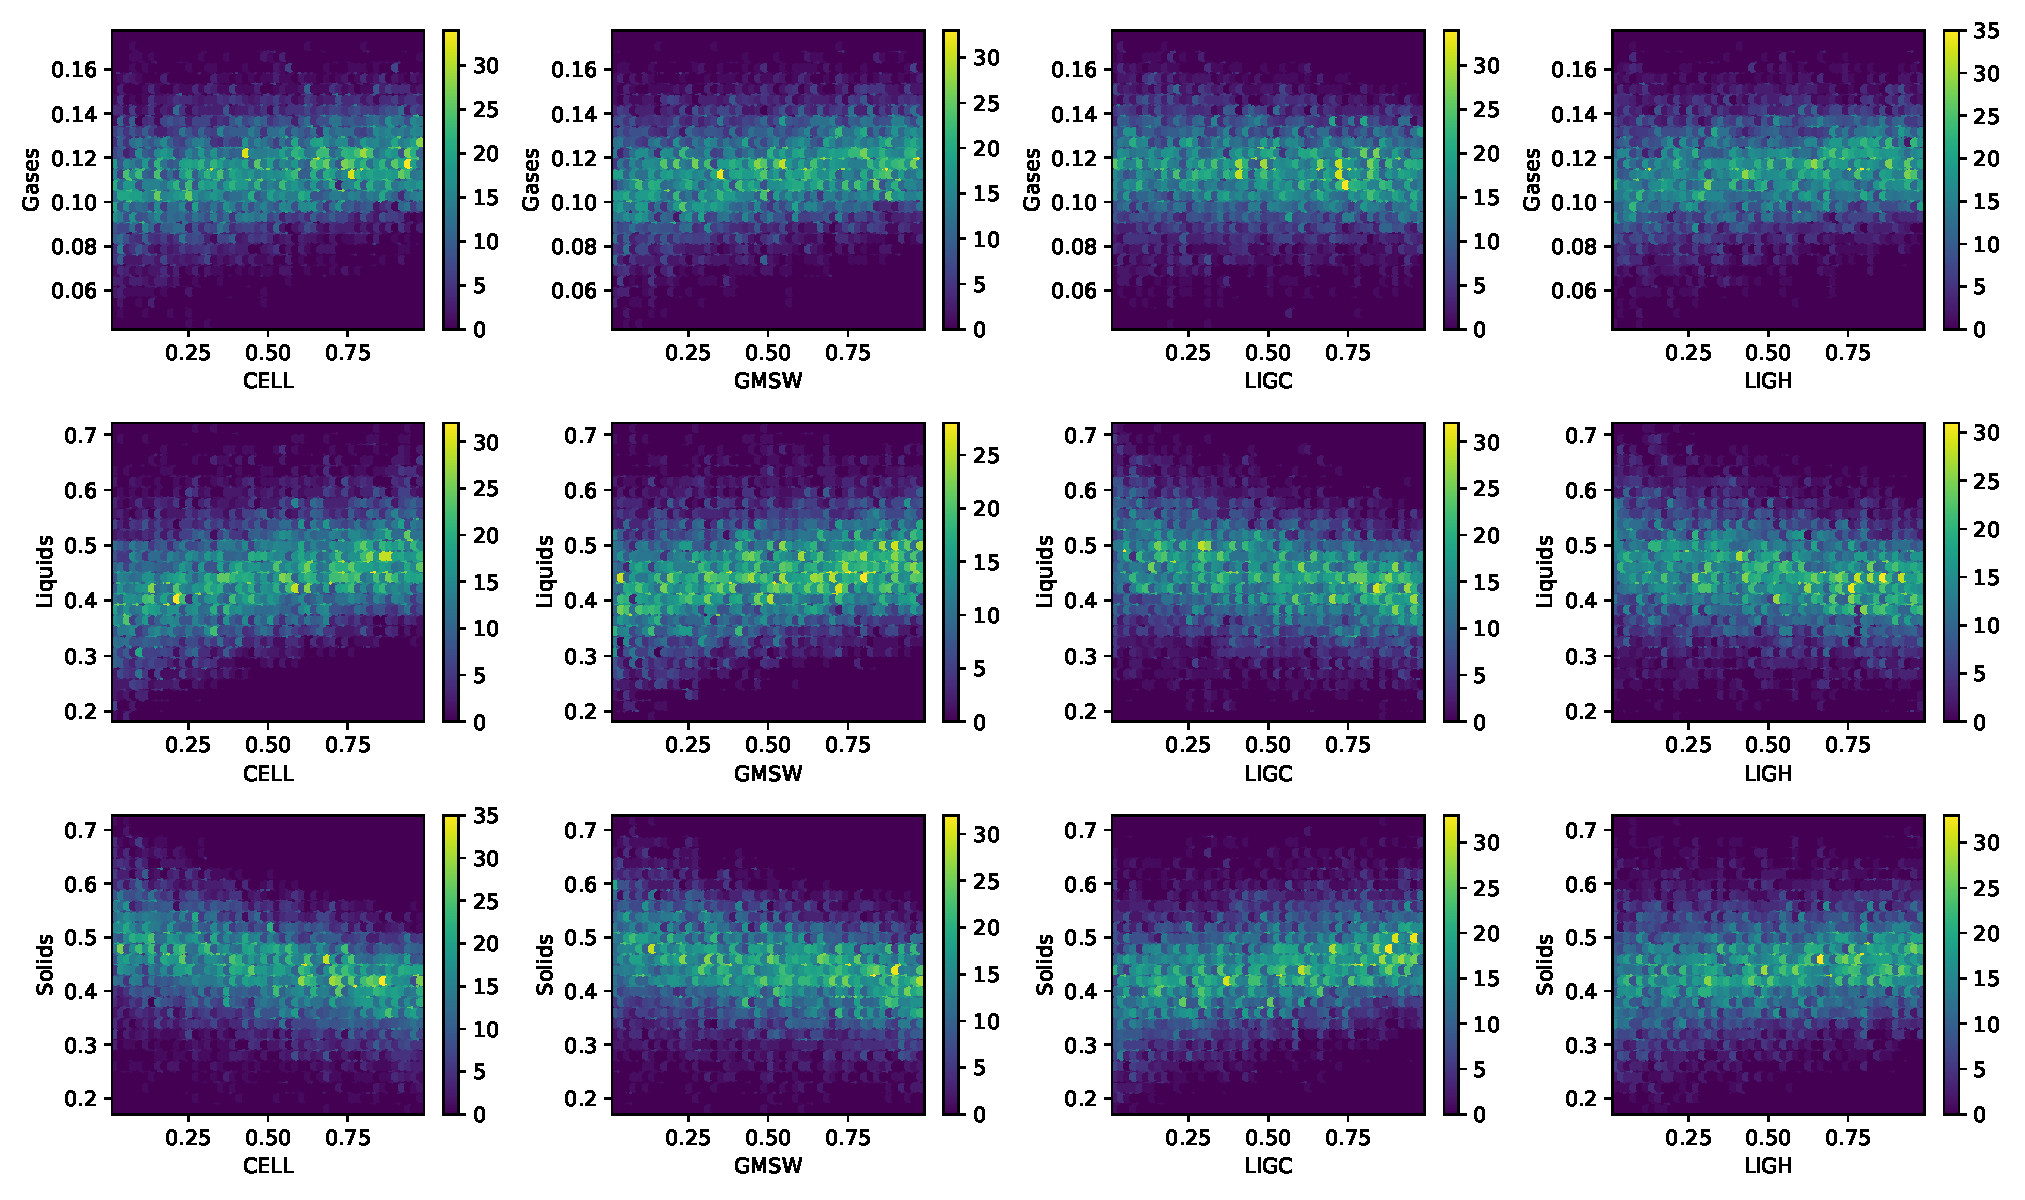
\includegraphics[width=1.3\textwidth]{figures/sa-hexbin1-n1000.pdf}}
    \caption{Batch reactor results for cellulose, hemicellulose (GMSW), carbon-rich lignin (LIGC), and hydrogen-rich lignin (LIGH) using 16,000 samples. Reaction time is 10 seconds at 773.15 K and 101,325 Pa. Colorbar represents bin count.}
\end{figure}

\begin{figure}[H]
    \centering
    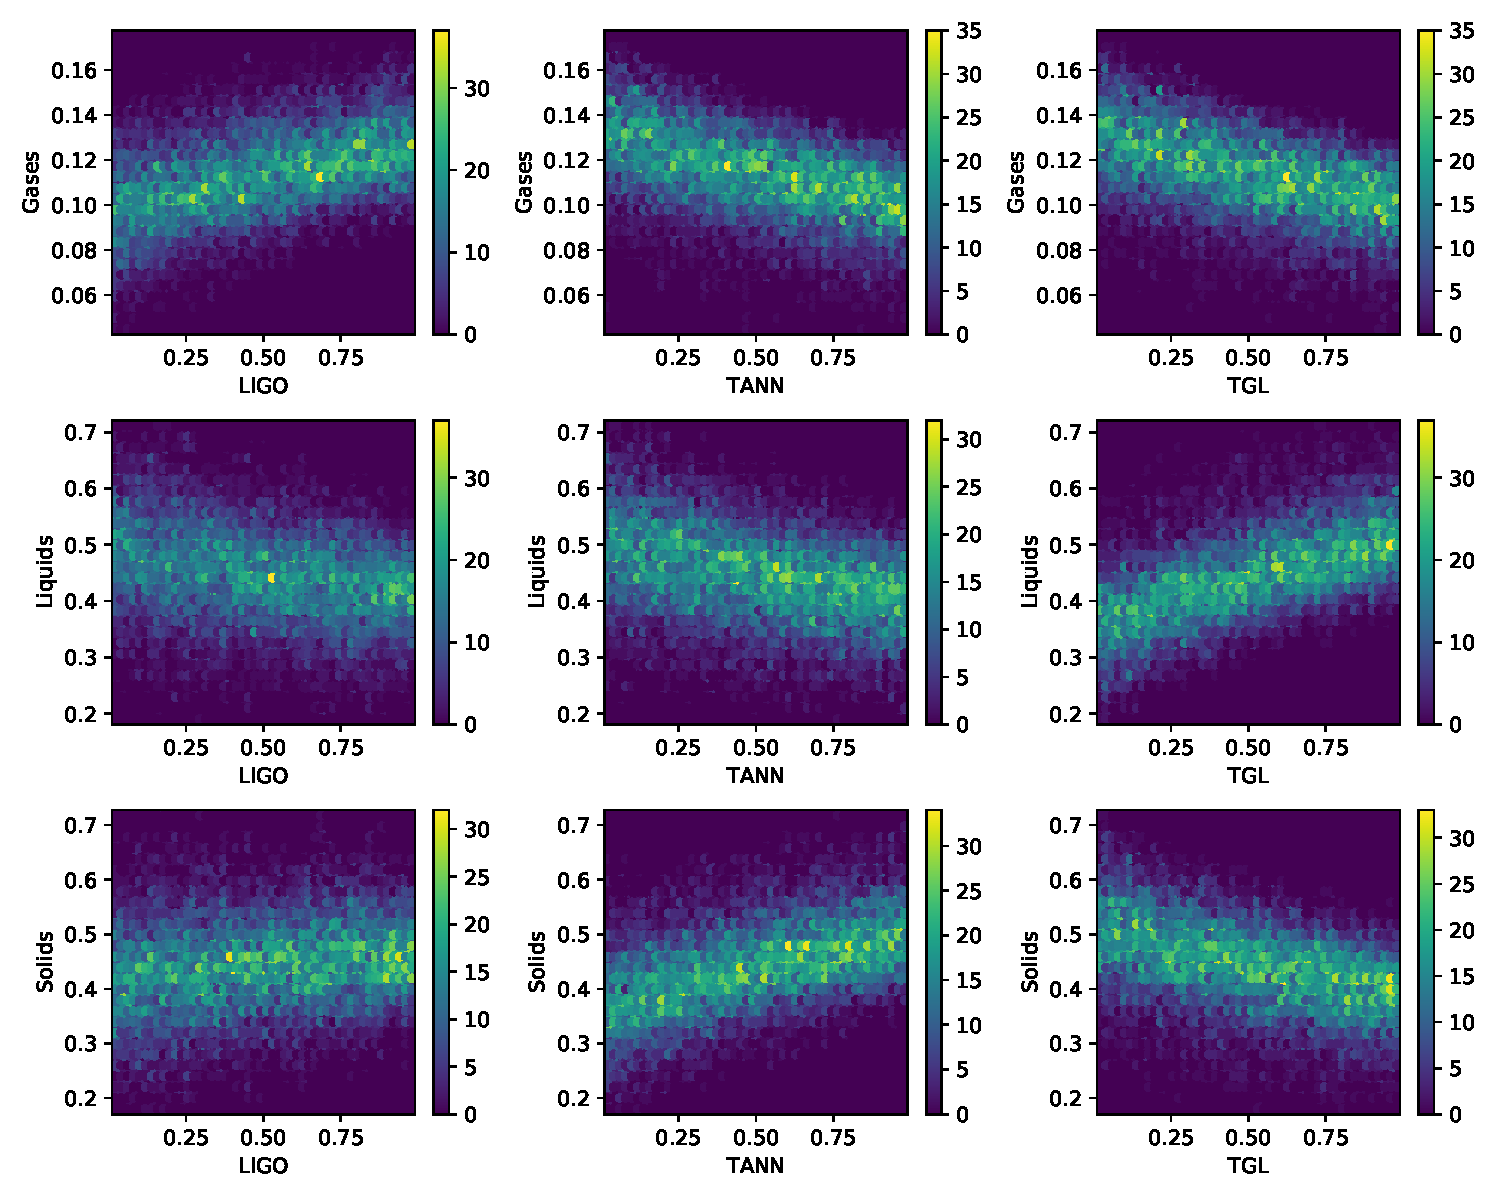
\includegraphics[width=\textwidth]{figures/sa-hexbin2-n1000.pdf}
    \caption{Batch reactor results for oxygen-rich lignin (LIGO), tannins (TANN), and triglycerides (TGL) using 16,000 samples. Reaction time is 10 seconds at 773.15 K and 101,325 Pa. Colorbar represents bin count.}
\end{figure}

\begin{figure}[H]
    \centering
    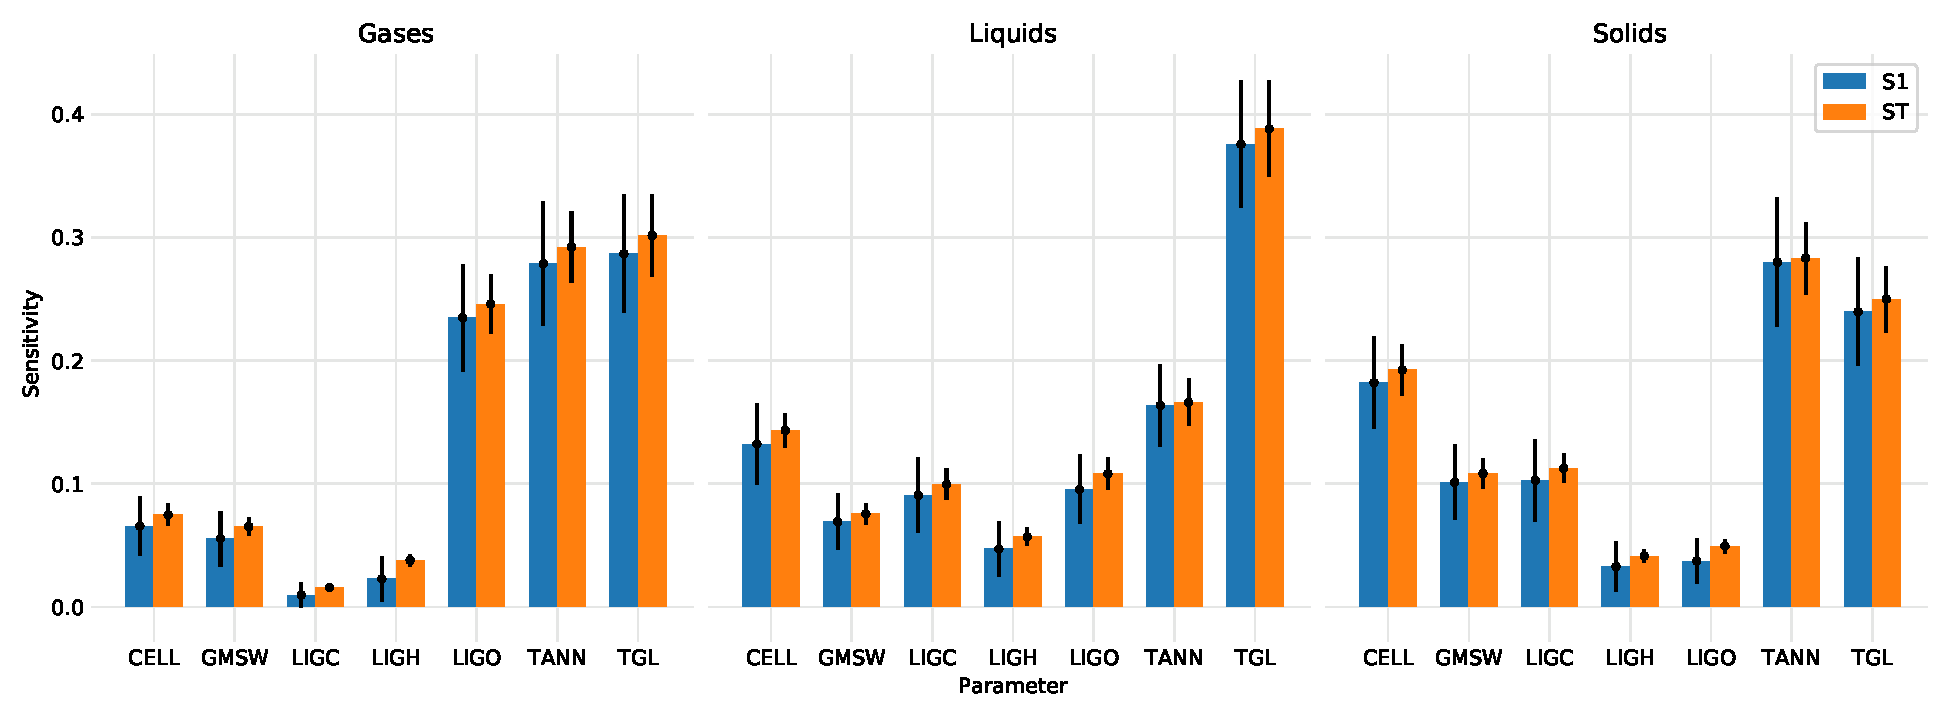
\includegraphics[width=\textwidth]{figures/sa-bar-n1000.pdf}
    \caption{First-order (S1) and total-order (ST) Sobol indices for biomass composition with reactants grouped as gases, liquids, and solids using 16,000 samples.}
\end{figure}

% !TEX root = ../main.tex

\section{Conclusions}

Here.

% !TEX root = ../main.tex

\section{Source code}

The Python code used to develop the models and generate results discussed in this paper is available on GitHub at \url{https://github.com/ccpcode/nrel-efr}.

% !TEX root = ../main.tex

\appendix

\section{Appendix}

\subsection{Sensitivity analysis}

\begin{figure}[H]
    \centering
    \makebox[\textwidth][c]{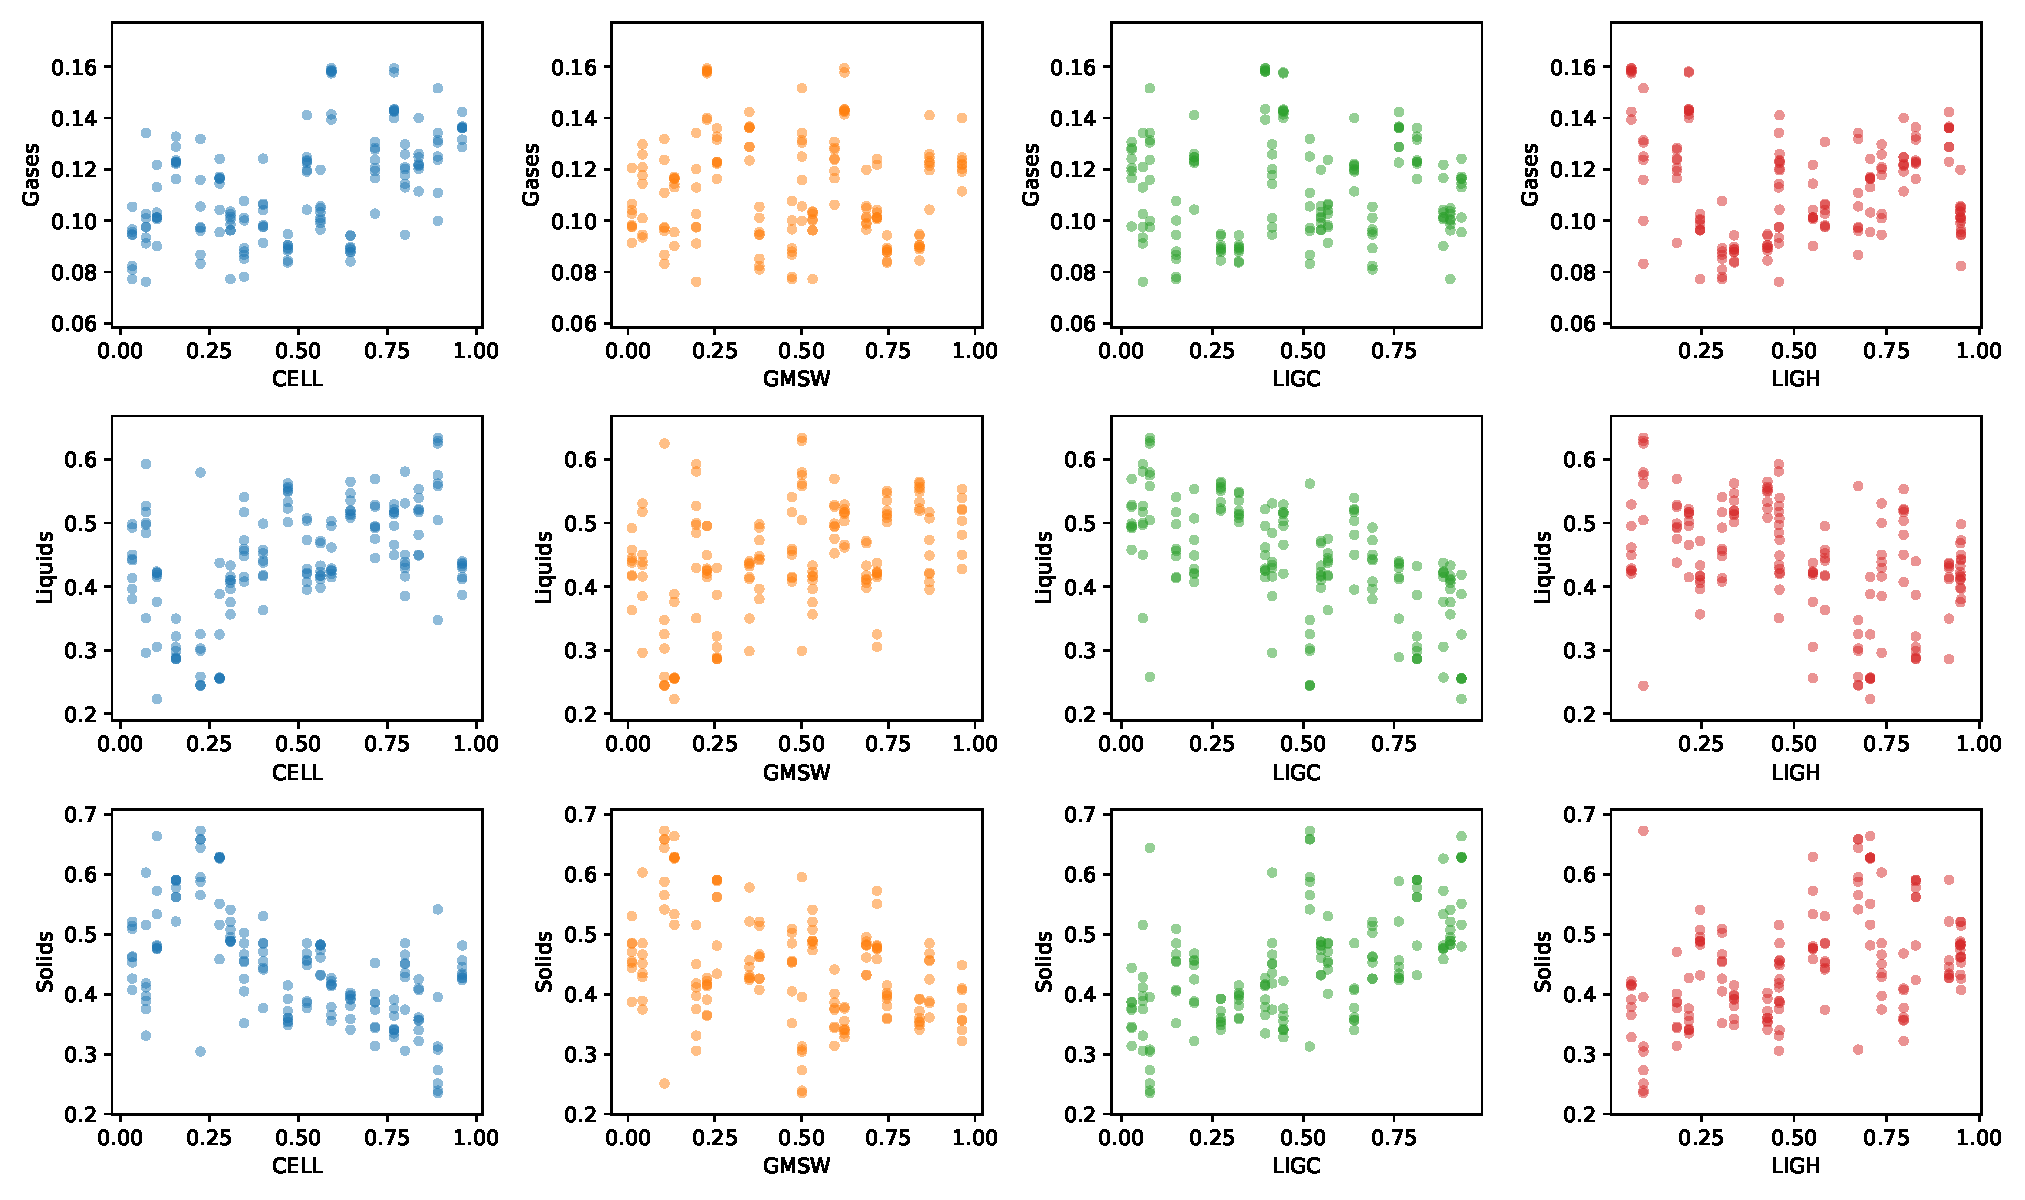
\includegraphics[width=1.3\textwidth]{figures/sa-scatter1-n10.pdf}}
    \caption{Batch reactor results for cellulose, hemicellulose (GMSW), carbon-rich lignin (LIGC), and hydrogen-rich lignin (LIGH) using 160 samples. Reaction time is 10 seconds at 773.15 K and 101,325 Pa.}
\end{figure}

\begin{figure}[H]
    \centering
    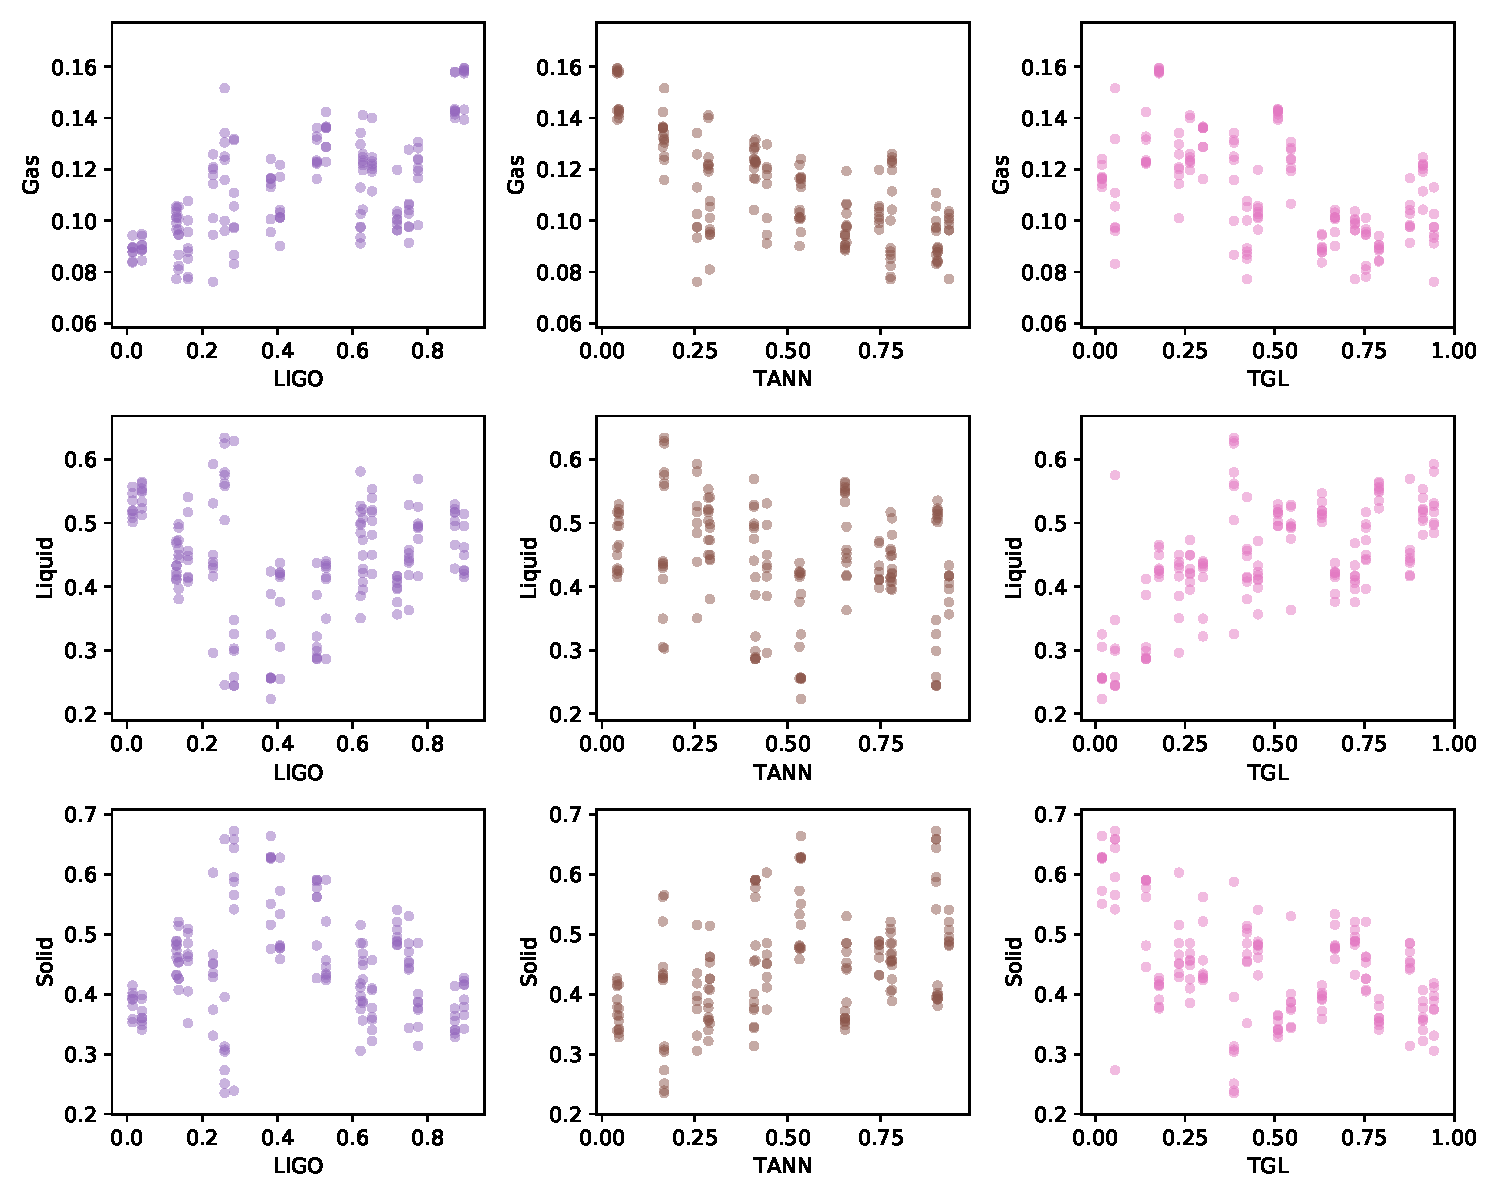
\includegraphics[width=\textwidth]{figures/sa-scatter2-n10.pdf}
    \caption{Batch reactor results for oxygen-rich lignin (LIGO), tannins (TANN), and triglycerides (TGL) using 160 samples. Reaction time is 10 seconds at 773.15 K and 101,325 Pa.}
\end{figure}

\begin{figure}[H]
    \centering
    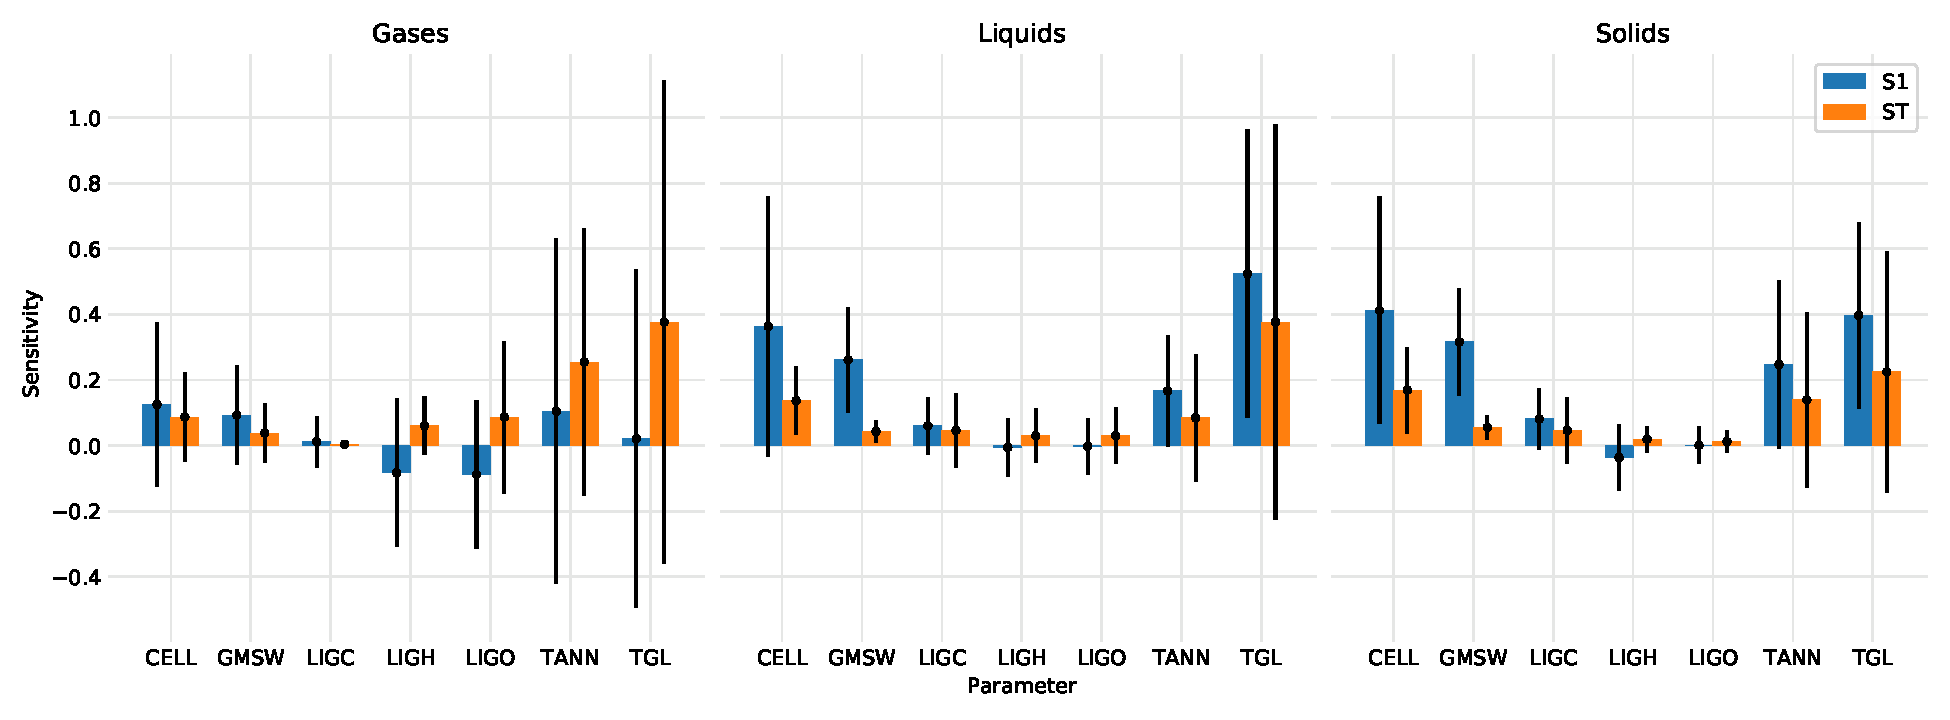
\includegraphics[width=\textwidth]{figures/sa-bar-n10.pdf}
    \caption{First-order (S1) and total-order (ST) Sobol indices for biomass composition with reactants grouped as gases, liquids, and solids using 160 samples.}
\end{figure}


\printbibliography
\addcontentsline{toc}{section}{References}

\end{document}
